In this section, we present an adaptive and interpretable detection framework (AID) designed for SCADA-based industrial systems with streaming IoT devices. Our approach is rooted in the foundational concepts discussed in Preliminaries~\ref{Preliminaries}. We systematically leverage these theoretical building blocks to introduce our method in a coherent manner.

Our approach begins by modeling the system as a dynamic multivariate normal distribution, allowing it to effectively handle pervasive nonstationary effects and interactions that impact industrial processes. We address several critical factors, such as change points, concept drift, and seasonal effects. Our primary contribution is the integration of an adaptable self-supervised system with root cause identification and dynamic operating limits setting. This unique combination empowers our online statistical model to diagnose anomalies through three distinct mechanisms.

Firstly, we employ conditional probability calculations to assess the normality of the system's operating conditions. This step ensures that our method identifies outliers within individual signal measurements and interprets the root causes of anomalies, facilitating faster and more precise diagnoses. Secondly, we detect abrupt changes due to concept drift, serving for faster adaptation to new operating conditions without human intervention. Thirdly, we harness interpretability as a tool to establish dynamic operating limits. These adaptive limits enable our framework to seamlessly integrate with existing SCADA-based infrastructure, a substantial advantage over existing solutions.

We have structured the subsequent sections to delve into the details of our proposed methodology by the logical flow of data. The upcoming subsection will cover the anomaly detection mechanism, followed by sections on online training and adaptation. The next subsection will describe dynamic operating limits setting, followed by diagnostic capabilities. Lastly, we describe how those parts converge into a diagnostic tool. For a schematic representation of our proposed method, with a highlighted subsection attribution, please refer to Figure~\ref{fig:method}. For a concise technical representation of our proposed method, please refer to Algorithm~\ref{alg:detector}.

\begin{figure}[htbp]
  \centering
  \resizebox{\linewidth}{!}{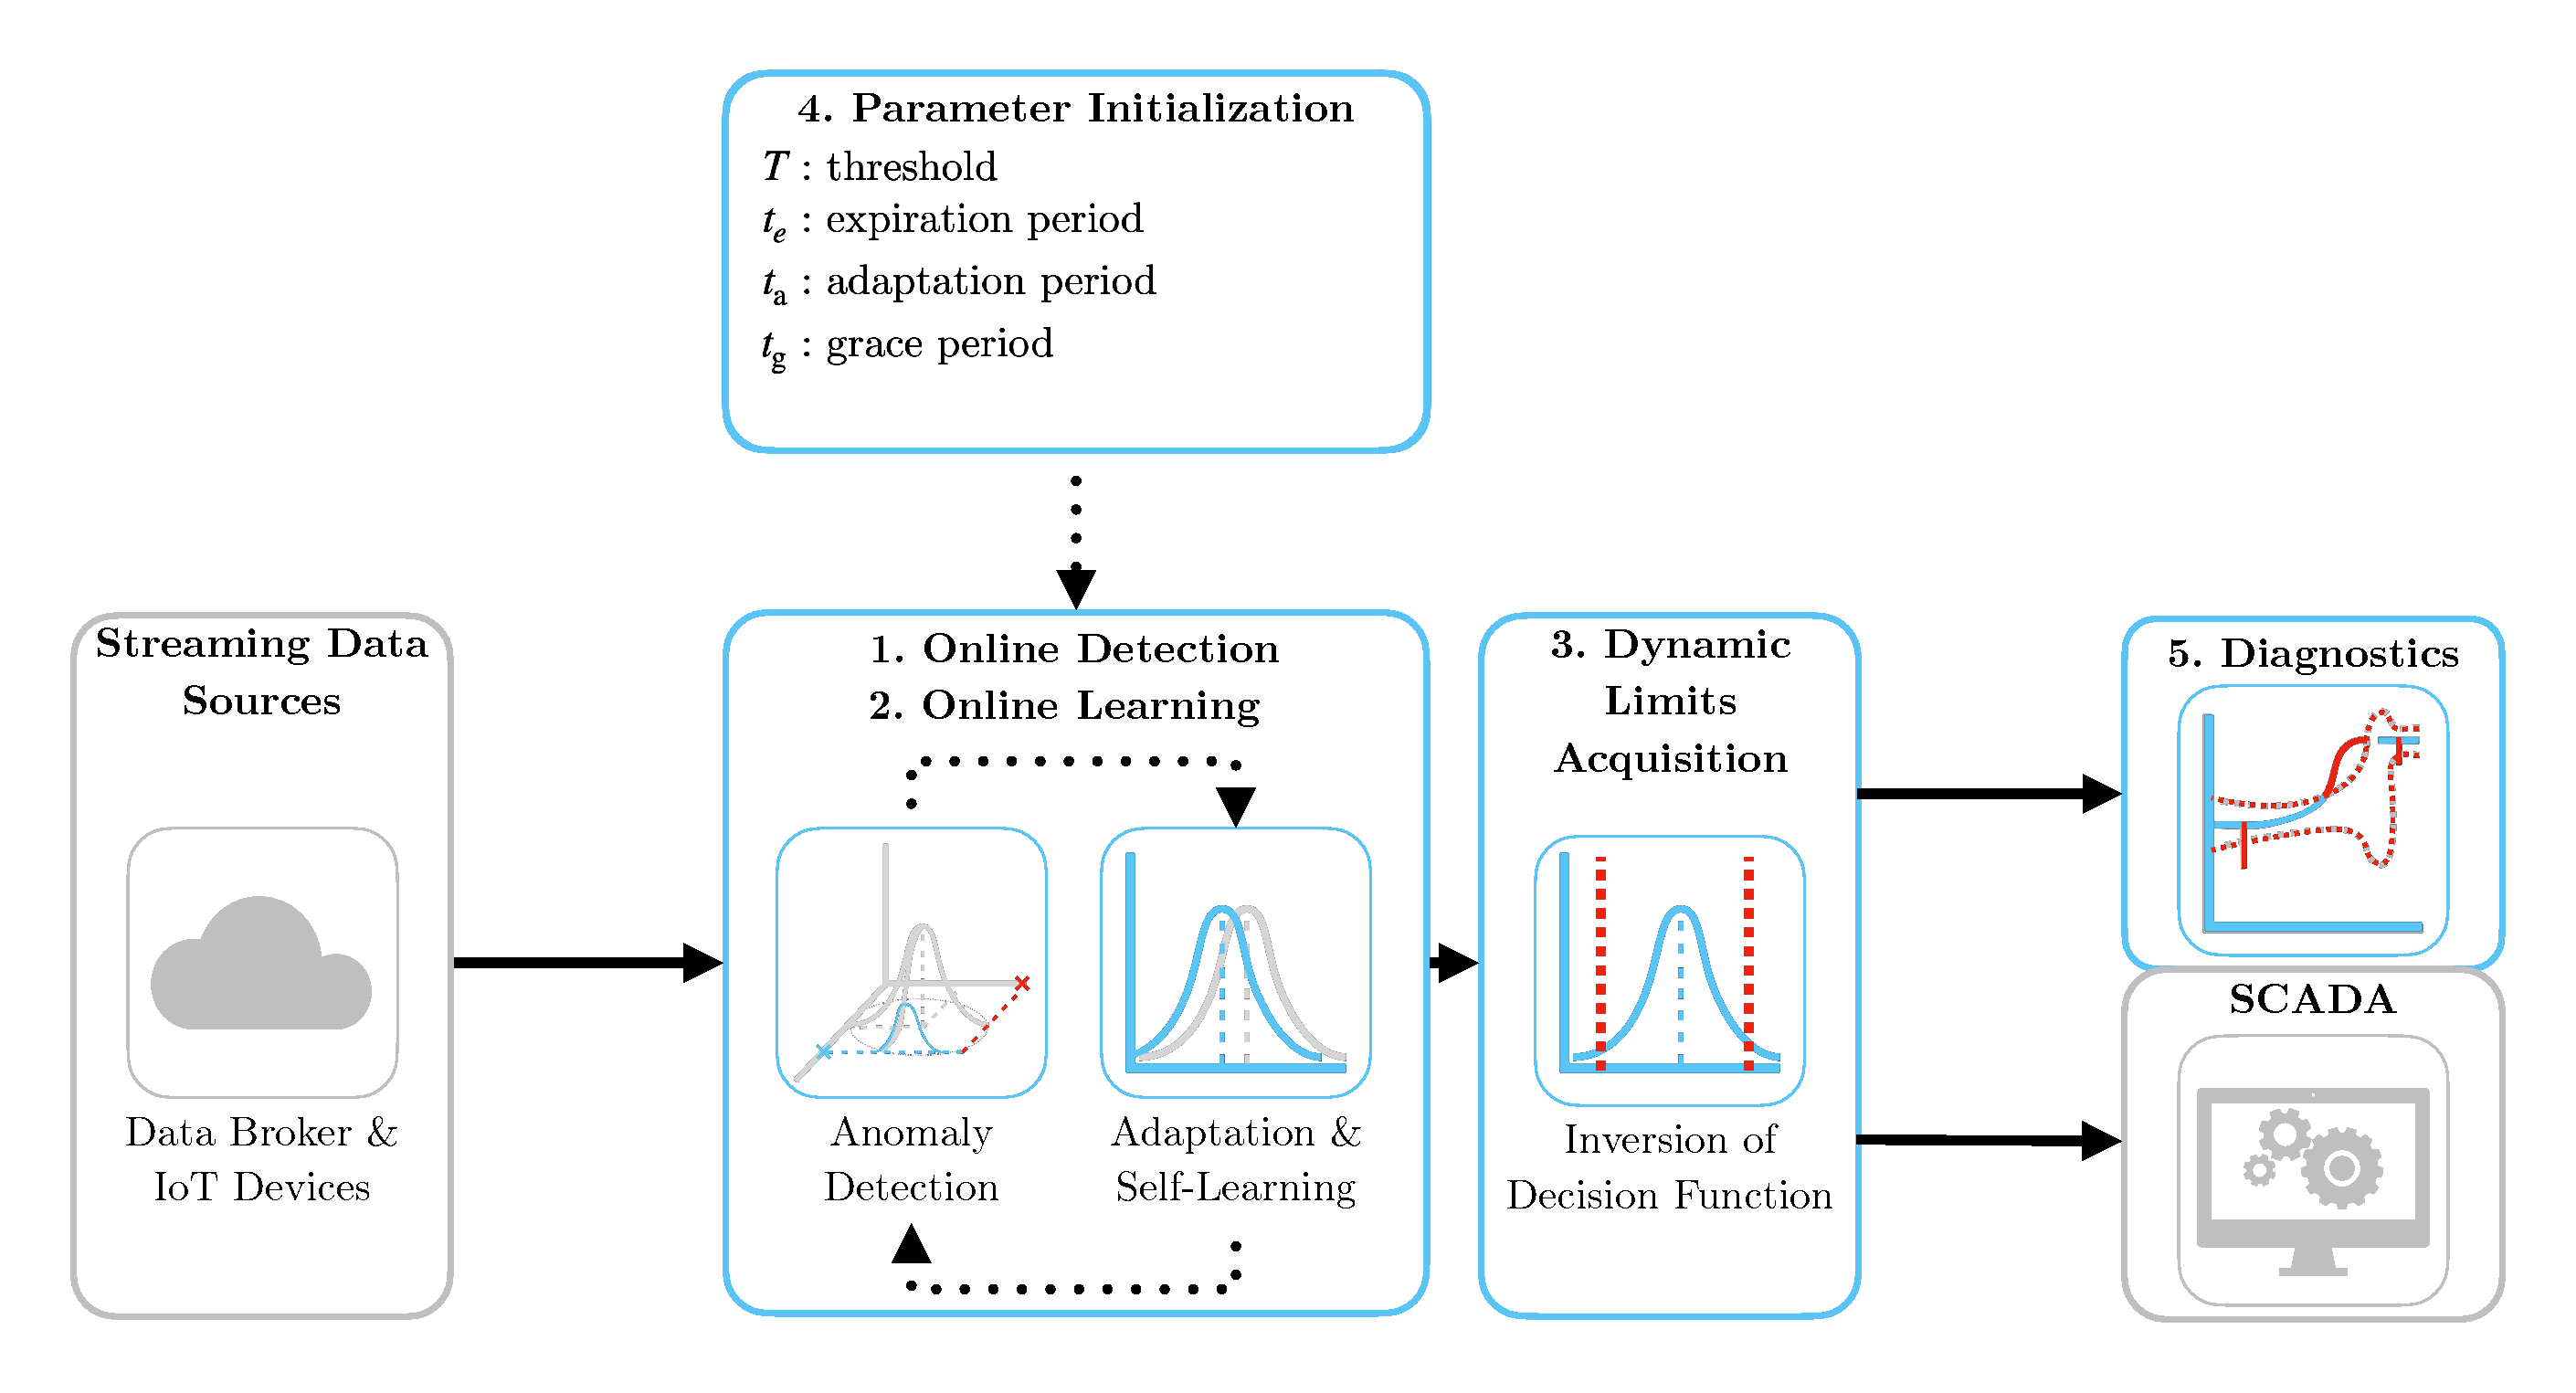
\includegraphics{figures/proposed_method.pdf}}
  \caption{Schematic representation of the proposed method AID with parameter initialization. Colored boxes represent steps described within the subsection.}
  \label{fig:method}
\end{figure}

\subsection{Online detection}\label{detect}
In the online detection phase, AID distinguishes between normal and anomalous observations based on the model of the system's normal behavior. The detection pipeline is event-triggered upon the arrival of a new set of measurements.

To initiate the process, AID computes the properties of the conditional distribution based on the current observations given the dynamic joint normal distribution. These calculations are performed for each element of the process observation vector $\boldsymbol{x}_i$ at time instance $i$. Specifically, we calculate the conditional mean using \eqref{eq:cond_mean} and the conditional variance using \eqref{eq:cond_var} for elements of $\boldsymbol{x}_i$. These computations yield univariate conditional distributions for individual signals and features. These conditional distributions play a crucial role in assessing the abnormality of signals and features concerning their relationships with other elements of $\boldsymbol{x}_i$. Consequently, AID inherently considers the interactions between input signals and features.

The determination of anomalous behavior is influenced by the parameter $T$, which is a user-defined hyperparameter representing a probabilistic threshold that sets the boundary between normal and anomalous behavior. Details regarding the selection of an appropriate value for $T$ are discussed in Subsection \ref{init}. Whenever an anomaly is detected within one of the signals or features, it triggers an alert regarding the overall system's anomalous behavior, as described in \eqref{eq:anomaly}. Nevertheless, individual determinations of anomalies serve as a diagnostic tool for isolating the root causes of anomalies, as further discussed in Subsection \ref{diagnosis}.

The proposed mechanism is applicable to both point anomalies and collective anomalies. In the case of collective anomalies, their duration and deviation may serve as precursors to concept drift in the system. To identify concept drift, we introduce a parameter adaptation period $\ui{t}{a}$. Given the predicted system anomaly state from \eqref{eq:anomaly} as $y_i$ over a window of past observations \(\boldsymbol{y}_i=\{y_{i-\ui{t}{a}},...,y_{i}\}\) bounded by $\ui{t}{a}$, the following test determines anticipated change points:

\begin{equation}
  {\frac{\sum_{y\in \boldsymbol{y}_i}y}{n(\boldsymbol{y}_i)}} > T\text{.}\label{eq:changepoint}
\end{equation}

Here, \(n(\boldsymbol{y}_i)\) denotes the dimensionality of \(\boldsymbol{y}_i\). The logic behind \eqref{eq:changepoint} is that over an adaptation period $\ui{t}{a}$, change points can be distinguished from collective anomalies and point anomalies due to their minimum duration, while $T$ allows for some overlap with previous normal conditions.

Our framework anticipates unexpected novel behavior, including non-uniformities in sampling. Assuming that the distribution of sampling times remains stable over the long term, we can employ equivalent steps on the observed time between samples to discriminate signal loss from long-term anomalous network events.

\subsection{Online learning}\label{train}
AID's training process follows an incremental self-learning approach, allowing for online model updates as new samples arrive. Self-learning, in this context, focuses on selecting only relevant data for training to maintain the model's long-term relevancy and stability. This approach proves particularly valuable in handling streaming data, where human supervision can introduce significant computational delays, affecting response time in a sequential setting.

In online anomaly detector training, regardless of the type of supervision, the learning is typically built upon observations of the normal state. We introduce a grace period denoted as $\ui{t}{g}$ to enable model calibration in the initial stages after deployment. During this period, when normality in samples is expected, the model learns from all observations. Subsequently, self-supervised and unsupervised detectors are expected to make autonomous decisions.

However, in the case of industrial systems, the drifts in the concept might often render the normal state anomalous, slowing down or preventing adaptation completely. This is particularly true for the case of seasonal effects, where the system is expected to operate in a different mode for a certain period of time. To address this issue, AID's adaptation incorporates two self-supervised mechanisms.

Firstly, the model is updated if the observation at time instance \(i\) is marked normal in the detection phase. In the case of a dynamic multivariate probability distribution, the updated parameters are $\boldsymbol{\mu_i}$ and $\boldsymbol{\Sigma_i}$ at time instance \(i\). Update of the mean vector $\boldsymbol{\mu_i}$ and covariance matrix $\boldsymbol{\Sigma_i}$ is governed by Welford's online algorithm using equation \eqref{eq:runmean} and \eqref{eq:runvar} respectively. Samples beyond the expiration period $\ui{t}{e}$, discussed further in Subsection \ref{init}, are disregarded during the second pass. The effect of expired samples is reverted using inverse Welford's algorithm for mean \eqref{eq:revmean} and variance \eqref{eq:revvar}, accessing the data in the bounded internal buffer. For more details, refer to Subsection \ref{AA:InvWelford}.

The second mechanism, which enables adaptation to anomalous samples, relies on changepoint detection. This mechanism operates under the assumption that detected changepoints represent new operational states with limited overlap with the previous ones, as specified in Equation \ref{eq:changepoint}. It facilitates rapid adaptation to evolving data patterns without the need for human intervention. The selection of the adaptation period $\ui{t}{a}$, as discussed further in Subsection \ref{init}, is thus crucial for determining the speed of adaptation or the potential mitigation of the second adaptation mechanism.

To anticipate potential deviations from sampling uniformity, we calculate the cumulative distribution function (CDF) over the univariate normal distribution of sampling. We operate under the assumption that, over the long term, the distribution of sampling times remains stable, employing a one-pass update mechanism of \eqref{eq:runmean} and \eqref{eq:runvar}, for efficiency. To proactively detect subtle changes in sampling patterns, self-supervised learning is employed, leveraging anomalies weighted by the deviation from $(1 - F(x_i; \mu, \sigma^2))$ for training.

\subsection{Dynamic limits acquisition}\label{limits}
As we wrote in the subsection Practical Impact \ref{par:practical_impact}, the monitoring mechanisms of SCADA readily depend on the upper and lower operating limits of individual parameters of the system. In the case of industrial systems, these limits are often defined by the sensor's designed limits and the system dynamics. These limits are typically static and do not account for the dynamically changing conditions. Our proposed method AID is capable of setting dynamic operating limits, thus allowing integration into the existing SCADA-based infrastructure.

The threshold $T$ applied on the dynamic multivariate normal distribution creates a confidence hyperellipse at $T$ probability level. Such a hyperellipse would not allow to effectively bound individual signals as it depends on values that other jointly distributed variables take. Nevertheless, by computing the conditional for process observation vector $\boldsymbol{x}_i$ at time instance $i$, we can compute the conditional density function for individual signals. By applying threshold $T$ on individual conditional probabilities, we establish a hypercube defined by lower and upper threshold values, denoted as $\ui{\boldsymbol{x}}{l}$ and $\ui{\boldsymbol{x}}{u}$, respectively. These thresholds are derived from \eqref{eq:thresh_low} and \eqref{eq:thresh_high}, incorporating updated model parameters. Lower and upper thresholds play a pivotal role as dynamic operating limits. They may be used as an addition to static operating limits used by monitoring systems in SCADA, accounting for spatial factors, such as multipoint measurements, temporal factors, such as aging, and actual environmental conditions that influence sensor operation. Moreover, any violation of the limits is also detected as an anomaly.

\subsection{Diagnostics}\label{diagnosis}
One of the crucial aspects of diagnostics is root cause isolation. Using the ability to detect anomalies in individual signals and features, AID is capable of isolating the root cause of anomalies with consideration of their mutual relationships. This is achieved by computing the conditional probability of individual signals and features given the rest of the process observation vector $\boldsymbol{x}_i$ at time instance $i$. The dynamic process limits further enhance the diagnosis by providing the context of the anomaly, including the extent of deviation from normal operation and the direction of the deviation. The proposed diagnostic mechanism is particularly useful in the case of collective anomalies, where the unified direction of deviations is expected. AID's interpretability is an asset for domain experts to understand why certain anomalies are flagged and enables operators to assess the system's state by visualizing limits and deviations, thus detecting the speed at which the process variable approaches the limits before an anomaly occurs.

\subsection{Model Parameters Initialization}\label{init}
The model initialization is governed by defining two required hyperparameters of the model: the expiration period ($\ui{t}{e}$) and the threshold ($T$). The expiration period determines the window size for time-rolling computations, impacting the proportion of outliers within a given timeframe and directly influencing the relaxation (with a longer expiration period) or tightening (with a shorter expiration period) of dynamic signal limits. Additionally, we introduce a grace period $\ui{t}{g}$, which defaults to $ui{t}{e}$, allowing for model calibration. During this grace period, system anomalies are not flagged to prevent false positives and speed up self-supervised learning, introduced in Subsection \ref{train}. $\ui{t}{g}$ can take any value smaller than $ui{t}{e}$, if the detection must be delivered fast after intergration. The length of the expiration period inversely correlates with the model's ability to adapt to sudden changes. The adaptation and detection of significant drifts in the data-generating process, such as changes in central tendency, is managed through the adaptation period $\ui{t}{a}$. A shorter $\ui{t}{a}$ results in faster adaptation to new operating conditions, while making the system vulnerable to prolonged collective anomalies. A longer $\ui{t}{a}$ results in slower adaptation to significantly deviating new operations, but allows longer alerts regarding collective anomalies. In most cases, $\ui{t}{a} = 1/4\ui{t}{e}$ offers optimal performance.

As a general rule of thumb, expiration period $\ui{t}{e}$ should be determined based on the slowest observed dynamics within the multivariate system. The threshold $T$ defaults to the three-sigma probability of $q$ in \eqref{eq:q}. Adjusting this threshold can fine-tune the trade-off between precision and recall. A lower threshold boosts recall but may lower precision, while a higher threshold enhances precision at the cost of recall. We recommend starting with the default values of other parameters and making adjustments based on real-time model performance, as the model's interpretability can reduce the time and effort required for fine-tuning. The presence of one non-default interpretable hyperparameter facilitates quick adaptation of AID in a broad range of use cases.

\begin{algorithm}[H]
  \caption{{Online Detection and Identification Workflow}} \label{alg:detector}
  \begin{algorithmic}[1]
    \renewcommand{\algorithmicrequire}{\textbf{Input:}}
    \renewcommand{\algorithmicensure}{\textbf{Output:}}
    \REQUIRE expiration period $\ui{t}{e}$
    \ENSURE system anomaly $y_i$, signal anomalies $\uis{\boldsymbol{y}}{s}{i}$, sampling anomaly $\uis{y}{t}{i}$, change-point $\uis{y}{c}{i}$, lower thresholds $\uis{\boldsymbol{x}}{l}{i}$, upper thresholds $\uis{\boldsymbol{x}}{u}{i}$,
    \\ \textit{Initialisation} :
    \STATE $i \leftarrow 1;~ n \leftarrow 1;~ T \leftarrow \eqref{eq:q};~ \boldsymbol{\mu} \leftarrow \boldsymbol{x_0};~ \boldsymbol{\Sigma} \leftarrow \mathbf{1}_{k \times k};~ \ui{\mu}{t} \leftarrow 0;~ \ui{\sigma}{t}^2 \leftarrow 1$;
    \STATE compute $F(\boldsymbol{x_0}; \boldsymbol{\mu}, \boldsymbol{\Sigma})$ using algorithm in \citet{Genz2000};
    \\ \textit{LOOP Process}
    \LOOP
    \STATE {$\boldsymbol{x}_i, t_i \leftarrow$ RECEIVE()};
    \STATE $\uis{\boldsymbol{y}}{s}{i} \leftarrow$ PREDICT($\boldsymbol{x}_i, T$) using \eqref{eq:anomaly_signal};
    \STATE $y_i \leftarrow$ PREDICT($\uis{\boldsymbol{y}}{s}{i}$) using \eqref{eq:anomaly};
    \STATE $\uis{\boldsymbol{x}}{l}{i}\text{, }\uis{\boldsymbol{x}}{u}{i} \leftarrow$ GET($T, \boldsymbol{\mu}, \boldsymbol{\Sigma}$) using \eqref{eq:thresh_low}, \eqref{eq:thresh_high};
    \STATE $\uis{y}{t}{i} \leftarrow$ PREDICT($t_i - t_{i-1}$) using \eqref{eq:anomaly_signal};
    \STATE {$\ui{\mu}{t}, \ui{\sigma}{t}^2 \leftarrow$ UPDATE($t_i - t_{i-1}, \ui{\mu}{t}, \ui{\sigma}{t}^2$) using \eqref{eq:runmean}, \eqref{eq:runvar}};
    \IF {\eqref{eq:anomaly} = 0 \OR \eqref{eq:changepoint}}
    \STATE {$\boldsymbol{\mu}, \boldsymbol{\Sigma} \leftarrow$ UPDATE($\boldsymbol{x}_i, \boldsymbol{\mu}, \boldsymbol{\Sigma}, n$) using \eqref{eq:runmean}, \eqref{eq:runvar}};
    \IF {\eqref{eq:changepoint}}
    \STATE $\uis{y}{c}{i} \leftarrow 1$;
    \ELSE
    \STATE $\uis{y}{c}{i} \leftarrow 0$;
    \ENDIF
    \STATE $n \leftarrow n + 1$;
    \FOR {$\boldsymbol{x}_{i-\ui{t}{e}}$}
    \STATE {$\boldsymbol{\mu}, \boldsymbol{\Sigma} \leftarrow$ REVERT($\boldsymbol{x}_{i-\ui{t}{e}}, \boldsymbol{\mu}, \boldsymbol{\Sigma}, n$) using \eqref{eq:revmean}, \eqref{eq:revvar}};
    \STATE $n \leftarrow n - 1$;
    \ENDFOR
    \ENDIF
    \STATE $i \leftarrow i + 1$;
    \ENDLOOP
  \end{algorithmic}
\end{algorithm}
